\scanpage{48}
% loc: item 4, heading and opening
\textcircled{4} \inserted{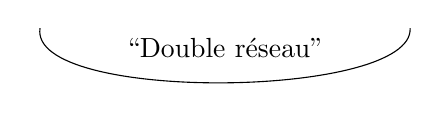
\begin{tikzpicture}[baseline=(n.base)]\node (n) {``\uline{Double réseau}''};\draw (-2.35,0.25) .. controls (-2.5,-0.7) and (2.4,-0.65) .. (2.35,0.25);\end{tikzpicture}} Supposons $S=\operatorname{Spec}k$, $k\subset\mathbb C$ extension \uline{algébrique} de $\mathbb Q$. Considérons le foncteur qui à $M$ associé
% loc: first labelled display
\begingroup\makeatletter\tagsleft@true\makeatother
\[
\bigl\{T_{\mathrm{DR}}(M),T_{\mathrm B}(M),\varphi_M\bigr\} \tag*{(4.1)}
\]
\endgroup
% loc: first comparison and question
où $\varphi:T_{\mathrm B}(M)\unsure{\otimes|\ominus}_{\mathbb Q}\mathbb C\simeq T_{\mathrm{DR}}(M)\unsure{\otimes|\ominus}_k\mathbb C$ ; ici, on ne considère pas $T_{\mathrm{DR}}(M)$ comme filtré, \deleted{et} ni $T_{\mathrm B}(M)$ muni d'une structure de Hodge. Ce foncteur est-il pl. fidèle ??

% loc: struck start and expression below it
\deleted{Il revient au $=$ de dire que}
\[
\deleted{T_{\mathrm R}(M)\cap T_{\mathrm{DR}}(M)}
\]
% loc: reduction to k with overbar
Il \deleted{est} aussitôt ramené au cas où $k=\overline{\mathbb Q}$. La question est alors équivalente à celle si le foncteur associant à $M$ le système
% loc: second labelled display
\begingroup\makeatletter\tagsleft@true\makeatother
\[
\bigl\{T_{\mathrm B}(M),\sigma\bigr\} \tag*{(4.2)}
\]
\endgroup
% loc: connexion paragraph
où $\sigma$ est la connexion canonique sur $T_{\mathrm B}(M)\otimes_{\mathbb Q}\mathbb C$, est pleinement fidèle : en effet, $\sigma$ et $T_{\mathrm{DR}}(M)$\inserted{$\subset T_{\mathrm B}(M)\unsure{\otimes|\ominus}_{\mathbb Q}\mathbb C$\unsure{,|;}} se déterminent mutuellement [$T_{\mathrm{DR}}(M)$ est l'ens. des éléments \inserted{de $T_{\mathrm B}(M)\otimes_{\mathbb Q}\mathbb C$} horizontaux pour $\sigma$ \ldots].
% loc: group description
Une autre façon de définir cette donnée, \inserted{$T_{\mathrm{DR}}\subset T_{\mathrm B}\otimes\mathbb C$,} quand on introduit le gpe de Galois $G=\underline{\operatorname{Aut}}_{\unsure{\ominus|\otimes}}(T_{\mathrm B}\deleted{\unsure{(M|M}})$ \deleted{\unsure{$\xi$} que \unsure{le}} ($M$ sous-$\otimes$-catégorie de type fini de la catégorie $\operatorname{Mot}(k)$) est la donnée de $\dot g\inG(\mathbb C)/G(\overline{\mathbb Q})$ ; si $V$ est un $G$-module (correspondant à un motif $\deleted{\unsure{V}}M$), alors
% loc: short note in left margin
\margin{\uline{NB} $G$ connexe}
% loc: lattice and inclusion
$T_{\mathrm{DR}}(M)$ n'est autre que le $\overline{\mathbb Q}$-réseau $g(V_{\overline{\mathbb Q}})\subset V\otimes_{\mathbb Q}\mathbb C$. Donc la question est simplement si pour tout $V$, l'inclusion
\[
V^G\subset V\cap g(\overline V)
\]
% loc: last lines
est une identité. [On peut supposer que $V$ est un module simple. [S'il est de dim. 1, c'est une puissance de Tate, et ça marche]] \deleted{Il revient au $=$ de}
% loc: line of dashes under the final cancellation
\par\hfill - - - - - - - - - -
% No watermark lettering securely recoverable on this image; the reading supplied by C remains an audit question.
% archive sheet number: 47

